\paragraph{QuizziPedia::Back-End::App::Models::LangModel}
\label{QuizziPedia::Back-End::App::Models::LangModel}
\begin{figure}
	\centering
	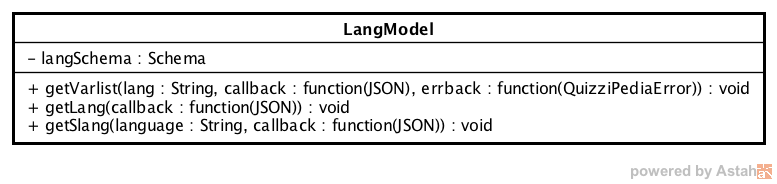
\includegraphics[scale=0.45]{UML/Classi/Back-End/QuizziPedia_Back-End_App_Models_langModel.png}
	\caption{QuizziPedia::Back-End::App::Models::LangModel}
\end{figure}
	\begin{itemize}
		\item \textbf{Descrizione} \\
		Classe che modella le informazioni riguardanti la lingua dell'applicazione;
		\item \textbf{Utilizzo} \\
		Viene utilizzata per scambiare memorizzare le traduzioni delle variabili che andranno visualizzate nella view\ped{G}.
		\item \textbf{Relazioni con altre classi} \\
			\begin{itemize}
				\item OUT LangController \\
				Classe che gestisce la logica applicativa riguardante la traduzione delle variabili;
			\end{itemize}
		\item \textbf{Attributi} \\
			\begin{itemize}
				\item \texttt{LangSchema : Schema} \\
				Questo campo rappresenta lo schema \textit{mongoose\ped{G}} per le variabili della lingua e prevede i seguenti attributi:
					\begin{itemize}
						\item \texttt{lang} di tipo \textit{String}, rappresenta la lingua scelta per l'applicazione;
						\item \texttt{eng} di tipo \texttt{Array}, contiene oggetti con coppie di tipo \texttt{String} che associano i nomi delle variabili alla loro traduzione in inglese;
						\item \texttt{ita} di tipo \texttt{Array}, contiene oggetti con coppie di tipo \texttt{String} che associano i nomi delle variabili alla loro traduzione in italiano;
					\end{itemize}
			\end{itemize}
		\item \textbf{Metodi}
			\begin{itemize}
				\item \texttt{+ getVarlist(lang: String, callback: function(JSON), errback: function(QuizziPediaError))} \\
				Metodo che permette di ritornare la traduzione delle variabili; \\
				\textbf{Parametri}:
					\begin{itemize}
						\item \texttt{lang: String} \\
						Rappresenta l'informazione che indica il set di traduzione da ritornare;
						\item \texttt{callback: function(JSON)} \\
						Rappresenta la \textit{callback\ped{G}} che verrà eseguita al termine dell'elaborazione nel caso non si verifichino errori durante l'esecuzione;
						\item \texttt{errback: function(QuizziPediaError)} \\
						Rappresenta la \textit{callback\ped{G}} che verrà eseguito al termine dell'elaborazione nel caso si verifichino errori durante l'esecuzione del metodo;
					\end{itemize}
			\end{itemize}
	\end{itemize}
	